
\documentclass{sigplanconf}

% The following \documentclass options may be useful:

% preprint      Remove this option only once the paper is in final form.
% 10pt          To set in 10-point type instead of 9-point.
% 11pt          To set in 11-point type instead of 9-point.
% authoryear    To obtain author/year citation style instead of numeric.

\usepackage{amsmath}

\usepackage{fancyvrb}
\usepackage{xspace}
\usepackage{graphicx}
\usepackage{../prov}
\usepackage{hyperref}

\hypersetup{
     colorlinks   = true,
     citecolor    = blue,
     linkcolor=blue,
     urlcolor=blue}
\usepackage{doi}


\newcommand{\RDF}{{\sc rdf}\xspace}
\newcommand{\REST}{{\sc rest}\xspace}
\newcommand{\POST}{{\sc post}\xspace}

\newcommand{\etal}{{\em et al.}\xspace}

\newcommand{\RESTful}{{\sc rest}ful\xspace}
\newcommand{\API}{{\sc api}\xspace}
\newcommand{\URL}{{\sc url}\xspace}
\newcommand{\HTTP}{{\sc http}\xspace}
\newcommand{\HTML}{{\sc html}\xspace}
\newcommand{\PROV}{{\sc prov}\xspace}
\newcommand{\PROVAQ}{{\sc prov-aq}\xspace}
\newcommand{\PROVDM}{{\sc prov-dm}\xspace}
\newcommand{\PROVN}{{\sc prov-n}\xspace}
\newcommand{\PROVO}{{\sc prov-o}\xspace}
\newcommand{\PROVJSON}{{\sc prov-json}\xspace}
\newcommand{\PROVXML}{{\sc prov-xml}\xspace}
\newcommand{\PROVSEM}{{\sc prov-sem}\xspace}
\newcommand{\PROVCONSTRAINTS}{{\sc prov-constraints}\xspace}

\newcommand{\rdfproperty}[2]{\href{#2}{#1}}

\newcommand{\provbook}[1]{\rdfproperty{\tt provbook:#1}{http://www.provbook.org/#1}}
\newcommand{\bk}[1]{\rdfproperty{\tt bk:#1}{http://www.provbook.org/ns/\##1}}
\newcommand{\now}[1]{\rdfproperty{\tt now:#1}{http://www.provbook.org/nownews/#1}}
\newcommand{\nowis}[1]{\rdfproperty{\tt is:#1}{http://www.provbook.org/nownews/is\##1}}
\newcommand{\nowpeople}[1]{\rdfproperty{\tt nowpeople:#1}{http://www.provbook.org/nownews/people/#1}}
\newcommand{\othernews}[1]{\rdfproperty{\tt other:#1}{http://www.provbook.org/othernews/#1}}
\newcommand{\policy}[1]{\rdfproperty{\tt pol:#1}{http://www.provbook.org/policyorg/#1}}
\newcommand{\gov}[1]{\rdfproperty{\tt gov:#1}{http://www.provbook.org/gov/#1}}
\newcommand{\govftp}[1]{\rdfproperty{\tt govftp:#1}{ftp://ftp.bls.gov/pub/special.requests/oes/#1}}
\newcommand{\prov}[1]{\rdfproperty{\tt prov:#1}{http://www.w3.org/ns/prov\##1}}
\newcommand{\ann}[1]{\rdfproperty{\tt ann:#1}{http://provenance.ecs.soton.ac.uk/annotate/ns/\##1}}
\newcommand{\foaf}[1]{\rdfproperty{\tt foaf:#1}{http://xmlns.com/foaf/0.1/\##1}}
\newcommand{\schema}[1]{\rdfproperty{\tt schema:#1}{http://schema.org/#1}}
\newcommand{\crypto}[1]{\rdfproperty{\tt crypto:#1}{http://www.w3.org/2000/10/swap/crypto\##1}}






\newcommand{\provstyMacro}[1]{{\tt \textbackslash prov{#1}}\xspace}
\newcommand{\latexMacro}[1]{{\tt \textbackslash#1}\xspace}
\newcommand{\provsty}{{\tt prov.sty}\xspace}

\begin{document}

\special{papersize=8.5in,11in}
\setlength{\pdfpageheight}{\paperheight}
\setlength{\pdfpagewidth}{\paperwidth}

\conferenceinfo{TAPP '15}{Month d--d, 2015, Edinburgh, Scotland, UK} 
\copyrightyear{2015} 
\copyrightdata{978-1-nnnn-nnnn-n/yy/mm} 
\thisdoi{nnnnnnn.nnnnnnn}

% Uncomment one of the following two, if you are not going for the 
% traditional copyright transfer agreement.

%\exclusivelicense                % ACM gets exclusive license to publish, 
                                  % you retain copyright

%\permissiontopublish             % ACM gets nonexclusive license to publish
                                  % (paid open-access papers, 
                                  % short abstracts)

\titlebanner{banner above paper title}        % These are ignored unless
\preprintfooter{short description of paper}   % 'preprint' option specified.

\title{\provTitle{Provenance of Publications: A PROV style for Latex}\footnotemark}


\authorinfo{\provAuthor{Luc Moreau}{http://orcid.org/0000-0002-3494-120X}}
           {\provOrganization{University of Southampton}{http://www.soton.ac.uk/}}
           {l.moreau@ecs.soton.ac.uk}


\authorinfo{\provAuthor{Paul Groth}{http://orcid.org/0000-0003-0183-6910}}
           {\provOrganization{Elsevier Labs}{http://labs.elsevier.com/}}
           {p.groth@elsevier.com}


\provLocation{http://eprints.soton.ac.uk/tbd/provenance.ttl}           
\maketitle\footnotetext{\label{prov:banner}\provBanner{http://eprints.soton.ac.uk/tbd/provenance.ttl}}
\provThis%
\provSpecialization{C4384149-0B34-4360-B2DA-A1AFFBB90188}% generic resource for all versions
\begin{abstract}
In general, the task of generating provenance is still tedious, and the community still lacks tools to generate provenance easily. In particular, when writing papers, researchers should be able to produce the provenance of their papers,  make it available online, and embed provenance metadata directly in their PDF file. To address this goal, we introduce \provsty, a \PROV style for \LaTeX, allowing \LaTeX\ source to be marked up, and associated provenance to be generated automatically. Provenance captured by this style currently includes: authors, organisations, funders, bibliographic citations, and embedded images. \PROV provenance is automatically generated and exported as a Turtle file; further, a link to a provenance resource can be embedded in PDF using the XMP metadata format.
\end{abstract}

%% \category{CR-number}{subcategory}{third-level}

%% % general terms are not compulsory anymore, 
%% % you may leave them out
%% \terms
%% term1, term2

\keywords
provenance,
\PROV,
latex style,
pdf embed,
xmp format,
tool

\section{Introduction}

Provenance, defined as a record that describes how entities, activities, and
agents have influenced a piece of
data~\cite{Moreau:prov-dm:20130430}, can help users make trust
judgements about data. \PROV is a set of W3C
specifications aiming to
facilitate the representation and exchange of provenance on the
Web. \PROV is domain-agnostic and is been applied to a wide range of
applications, including climate
assessment\footnote{\url{http://nca2014.globalchange.gov/report}},
legal notices\footnote{\url{https://www.thegazette.co.uk/}}.

While the provenance community has made substantial progress in terms
of understanding and standardising provenance, it is an unfortunate
reality that, due to the lack of easy tools, provenance still remains
beyond the reach of the general public.  For this paper's authors,
who are willing to work with leading-edge, non-mature technology, it is
a great frustation that provenance of their papers cannot be generated
automatically, and that best practice cannot be demonstrated to the
research community.  No more!

Publications already contain a lot of provenance information in
textual form, but it is not exposed in \PROV format: authorship,
institutions, sponsoring projects, included graphics, and
bibliography. The purpose is this work is to demonstratre how this
textual information can be marked up, so that \PROV can be generated
automatically and provenance metadata embedded in the PDF.  The
approach is implemented by a style \provsty for \LaTeX.  The interest
of the approach is that provenance is generated systematically, as
part of the typesetting process, for each version of the document
produced.

The purpose of this short paper is to outline the approach, to
describe the \LaTeX\ annotation macros and the
\PROVO-compliant~\cite{Lebo:prov-o:20130430} provenance they generate,
to explain the actual provenance generated for this document, and to
explain how provenance metadata can be embedded in the PDF file, by
exploiting the XMP metadata standard~\cite{Adobe_XMP_Spec_part1}. At
the same time, we are releasing \provsty on GitHub at \provstyurl.



\section{Author Guide}

The style was designed with a view to minimize author's work. The
adopted approach is to import the package, annotate the \LaTeX\ source
without having to duplicate information, generate the provenance on
the fly every time \LaTeX\ is run, and embed provenance information in
the PDF using XMP automatically.

In practice, the provenance file in Turtle
format~\cite{Lebo:prov-o:20130430} has to be deployed and made web
accessible. (This process is not handled by \provsty.)
Footnote~\ref{prov:banner} embeds in the text the location of the
provenance, for user consumption.



\subsection{Preamble}

The preamble must import the package \provsty.
\begin{verbatim}
\usepackage{prov}
\end{verbatim}
Whenever \LaTeX\ is run, (see Section~\ref{implementation:section}), a
unique identifier is created for the current document, and provenance
is generated in a separate file. This is being referred to as ``author'' mode.

Alternatively, using the optional ``publisher'' mode, provenance is no
longer computed, and annotations are simply ignored.

\begin{verbatim}
\usepackage[publisher]{prov}
\end{verbatim}


\subsection{Document Annotations}\label{annotations:section}

The \provsty package offers a series of macros that the author can use
to annotate \LaTeX\ documents, with a view of generating its \PROV
provenance. This section introduces the \provsty macros.  When
\provsty is used in publisher mode, these annotations have no
effect. In the rest of the section, we describe the macros
intuitively, and we illustrate the Turtle statements they generate.

\subsubsection{\provstyMacro{This} and \latexMacro{thisresource}}\label{this:macro}

The macro \provstyMacro{This} generates an \RDF description of the
current document as a \prov{Entity}.  The macro makes use of the
internal macro \latexMacro{thisresource} to obtain a URI Reference for
this document. The macro \latexMacro{thisresource} expands into a
string of characters. This macro would typically not be used by
authors, unless they program other \provsty related macros, or they
want to include the document's identifier in the text, as we did in
Footnote~\ref{prov:banner}.

At the beginning of the document, we expect the following annotations
to be inserted.

{\footnotesize
\begin{Verbatim}
\provThis
\end{Verbatim}
}

In response, the following Turtle statement is generated. For every
run of \LaTeX, a new identifier is generated, since the resulting PDF
is a new \prov{Entity}. To this end, we use a UUID generator.

{\footnotesize
\begin{Verbatim}[commandchars=\\\{\}]
\thisresourceShort  a prov:Entity .
\end{Verbatim}
}


\subsubsection{\provstyMacro{Author}}\label{author:macro}

The macro  \provstyMacro{Author} allows the author of the current document to be declared.
The macro takes two arguments: the first is the author's name, which
is associated with the author resource by the property \foaf{name},
whereas the second is a URI for the author.  In publisher's mode, this
macro expands to the author string, ignoring the second
argument. Typically, this annotation occurs inside the
\latexMacro{author} declaration for the paper.

{\footnotesize
\begin{Verbatim}
\provAuthor{Luc Moreau}%
           {http://orcid.org/0000-0002-3494-120X}
\end{Verbatim}
}

\noindent In response, the following Turtle statements are generated:

{\footnotesize
\begin{Verbatim}[commandchars=\\\{\}]
<http://orcid.org/0000-0002-3494-120X>
    a prov:Agent, prov:Person;
    foaf:name "Luc Moreau" . 
\thisresourceShort
    prov:wasAttributedTo 
    <http://orcid.org/0000-0002-3494-120X> .
\end{Verbatim}
}


\subsubsection{\provstyMacro{Organization}}\label{organization:macro}

The macro \provstyMacro{Organization} allows an author's organization
to be declared.
The macro takes two arguments, the first is the organization's name,
which is linked with property \foaf{name}, whereas the second is the
organization's URI.  In publisher's mode, this macro expands to the
organization string, ignoring the second argument.

{\footnotesize
\begin{Verbatim}
\provOrganization{University of Southampton}%
                 {http://www.soton.ac.uk/}
\end{Verbatim}
}

\noindent The following Turtle statements are generated:

{\footnotesize
\begin{Verbatim}[commandchars=\\\{\}]
<http://www.soton.ac.uk/>
   a prov:Agent, prov:Organization;
   foaf:name "University of Southampton" . 
\thisresourceShort
   prov:wasAttributedTo <http://www.soton.ac.uk/> .
\end{Verbatim}
}
  

\subsubsection{\provstyMacro{Title}}

The macro \provstyMacro{Title} allows a document title to be declared.

The macro takes a single argument: the title itself, which 
 is linked to this resource with the property \schema{headline}.
The macro expands to the title
string. Typically, this annotation
occurs inside the \latexMacro{title} declaration for the paper.

{\footnotesize
\begin{Verbatim}
\provTitle{A PROV style for latex}
\end{Verbatim}
}

\noindent In response, the following triple is generated:

{\footnotesize
\begin{Verbatim}[commandchars=\\\{\}]
\thisresourceShort
  schema:headline "A PROV style for latex" .
\end{Verbatim}
}

\subsubsection{\provstyMacro{Project}}\label{project:macro}


The macro \provstyMacro{Project} allows a sponsoring project to be declared.

The macro takes three arguments, the first is the project name, the
second is a URI for this resource, and the third is the funding
agency.  In publisher's mode, this macro expands to the project
string, ignoring the remaining two arguments.

{\footnotesize
\begin{Verbatim}
\provProject{SOCIAM}%
            {http://www.sociam.org/}%
            {http://www.epsrc.ac.uk/}
\end{Verbatim}
}

\noindent In response, the following Turtle statements are generated:

{\footnotesize
\begin{Verbatim}[commandchars=\\\{\}]
<http://www.sociam.org/> a prov:Agent;
   foaf:name "SOCIAM" ; 
   prov:actedOnBehalfOf <http://www.epsrc.ac.uk/> .
\thisresourceShort
     prov:wasAttributedTo <http://www.sociam.org/> .
\end{Verbatim}
}

\subsubsection{\latexMacro{includegraphics}, \provstyMacro{Include} and \provstyMacro{Resource}}\label{include:macro}

The macro \latexMacro{includegraphics} (from package graphicx) can be
used to include graphics in the current document.  Package \provsty
redefines the macro \latexMacro{includegraphics}, so as to
call \provstyMacro{Include}, a macro in charge of recording the
provenance of this inclusion: the current document is said to be
derived from the included resource.

The included resource is a file on the file system, so a third party
would typically not be able to access it directly. For this reason,
the macro \provstyMacro{Resource} allows for an online resource, copy
of the included file, to be declared.  Thus, the provenance of this
inclusion is modelled as follows: the current document was derived
from the included resource, itself an alternate of the online
resource.  For a third party to be able to check that the online
resource is a copy of the included one, \provsty computes the md5 hash
of the included file.

{\footnotesize
\begin{Verbatim}
\provResource{http://example.org/myfig.pdf}
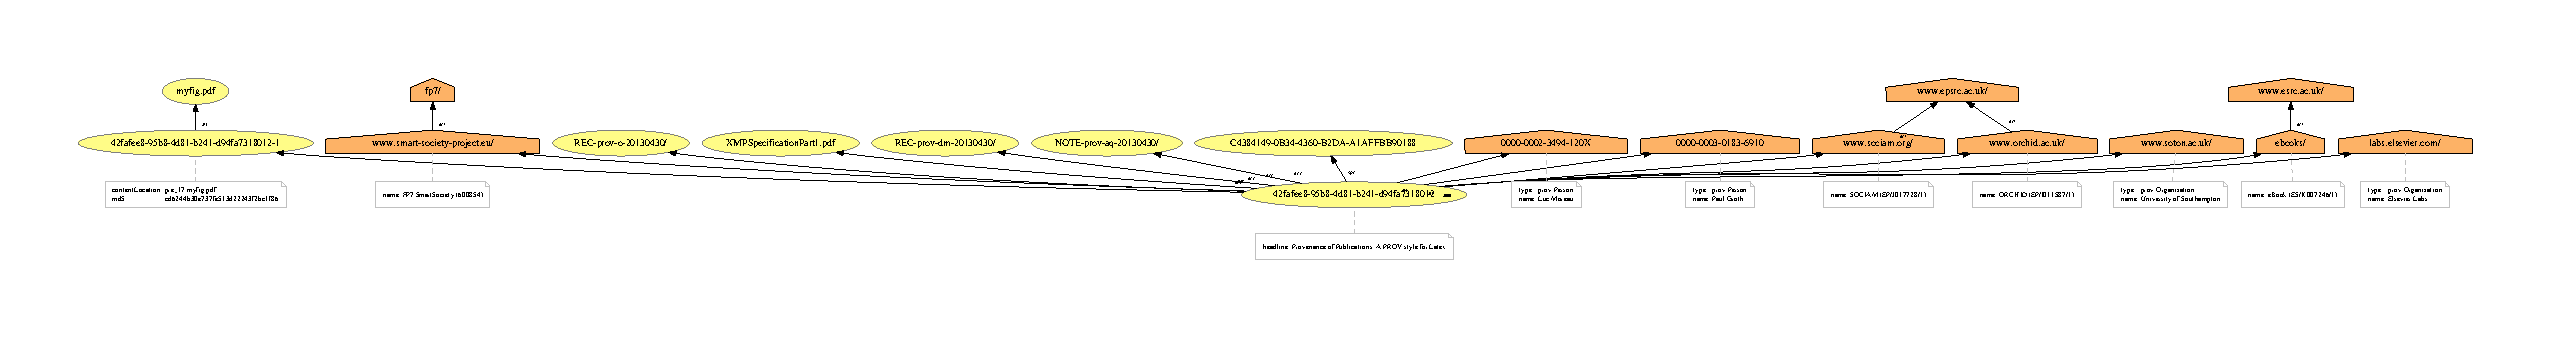
\includegraphics{myfig.pdf}
\end{Verbatim}
}

In response, the following Turtle statements are generated. A new
resource is introduced to represent the included file. Its md5 is
associated with property \crypto{md5}. Its local path on the
filesystem is asserted using property \schema{contentLocation}.

{\footnotesize
\begin{Verbatim}[commandchars=\\\{\}]
\thisresourceShort
  prov:wasDerivedFrom
  \thisresourceShortArg{1} .

\thisresourceShortArg{1}
       a prov:Entity ;
       schema:contentLocation <myfig.pdf> ;
       prov:alternateOf <http://example.org/myfig.pdf> ;
       crypto:md5 "b67f7e8398b175245b59511ee5aa362d" . 

<http://example.org/myfig.pdf>
       a prov:Entity . 
\end{Verbatim}
}




\subsubsection{\provstyMacro{Bibliography} and \provstyMacro{Citation}}\label{citation:macro}

The macro \provstyMacro{Bibliography} allows for provenance to be
generated for the bibliography. No further annotation is required, but
\provsty requires bibliographic entries to contain URIs or DOIs. The
corresponding macros \latexMacro{uri} and \latexMacro{doi}
are overriden, to call \provstyMacro{Citation}.

The following declaration is expected to be placed just before the
\LaTeX\ \latexMacro{bibliography} macro.

{\footnotesize
\begin{Verbatim}
\provBibliography
\end{Verbatim}
}

For instance, this document cites
\PROVDM~\cite{Moreau:prov-dm:20130430}, which leads to the following
Turtle statement, describing the dependency of this document on the \PROVDM resource.

{\footnotesize
\begin{Verbatim}[commandchars=\\\{\}]
\thisresourceShort
   prov:wasDerivedFrom
  <http://www.w3.org/TR/2013/REC-prov-dm-20130430/> . 
\end{Verbatim}
}



\subsubsection{\provstyMacro{Specialization}}\label{specialization:macro}

The macro \provstyMacro{Specialization} allows for a more general resource to be identified, representing all the variants of the current document.
Indeed, a given document may have multiple variants.  Not only we have various versions, but also there may be a pre-print version in an institutional repository, an editor-compiled version for the proceedings, and the final version published by the publisher. With \provstyMacro{Specialization}  generic version of the document can be hard-coded in the paper.

{\footnotesize
\begin{Verbatim}
\provSpecialization{C4384149-0B34-4360-B2DA-A1AFFBB90188}
\end{Verbatim}
}


In response, the following Turtle statement is generated, making use of the \prov{specializationOf} property.

{\footnotesize
\begin{Verbatim}[commandchars=\\\{\}]
\thisresourceShort
   prov:specializationOf
   ex:C4384149-0B34-4360-B2DA-A1AFFBB90188  .
\end{Verbatim}
}


\subsubsection{\provstyMacro{Embed} and \provstyMacro{Location}}

The macro \provstyMacro{Embed} allows for metadata about the
provenance to be inserted in the PDF document, using the XMP metadata
format~\cite{Adobe_XMP_Spec_part1}.  This command is expected to be
called as the last macro before the end of the document.  XMP supports
a subset of RDF/XML that does not appear to be expressive enough to
embed \PROV provenance directly. Instead, using the approach recommended
by \PROVAQ~\cite{Klyne:prov-aq:20130430}, a pointer to the provenance
is expressed, using the XMP format.


{\footnotesize
\begin{Verbatim}
\provLocation{http://example.org/provenance.ttl}
\provEmbed
\end{Verbatim}
}

In response, the following Turtle statements are generated, and
embedded as XMP metadata. The current resource has some provenance
\prov{has\_provenance} that can be found at the location provided by
macro \provstyMacro{Location}; this resource is known in that
provenance file as the resource object of \prov{has\_anchor}.

{\footnotesize
\begin{Verbatim}[commandchars=\\\{\}]
<>
 prov:has_anchor \thisresourceShort ;
 prov:alternateOf \thisresourceShort ;
 prov:has_provenance <http://example.org/provenance.ttl>.
\end{Verbatim}
}

As noted before, it is the author's responsibility to make the
provenance available online at the declared URI.

\subsection{Invocation}\label{implementation:section}

To run \LaTeX, one needs the option {\tt --shell-escape} to allow for
a UUID generator and the ProvToolbox's {\tt provconvert} to be called
during typesetting. (Note that this is not required when \provsty is
used in publisher mode.)


{\footnotesize
\begin{Verbatim}[commandchars=\\\{\}]
	pdflatex  --shell-escape prov-sty-tapp15.tex
\end{Verbatim}
}

\section{Provenance Modelling}

Section~\ref{annotations:section} lists the \provsty annotations and
includes snippets of \RDF generated by these. For this document, the
full provenance is displayed in Figure~\ref{prov:fig}. (Concretely,
this image was generated by converting the provenance of a previous
version of the document into PDF.)

\begin{figure*}[htb]
  \hspace{7cm}
  \setlength{\unitlength}{1cm}%
  \begin{picture}(0,0)
    %% this
    \put(1,2.5){\vector(1,0){4}}
    \put(5,2.7){\frame{\provstyMacro{This} (\ref{this:macro})}}
    %% author
    \put(1,5.0){\vector(1,0){4}}
    \put(5,5.2){\frame{\provstyMacro{Author} (\ref{author:macro})}}
    %% organisation
    \put(1,11.4){\vector(1,0){4}}
    \put(5,11.6){\frame{\provstyMacro{Organization} (\ref{organization:macro})}}
    %% project
    \put(1,7.4){\vector(1,0){4}}
    \put(5,7.6){\frame{\provstyMacro{Project} (\ref{project:macro})}}
    %% citation
    \put(1,-2.6){\vector(1,0){4}}
    \put(5,-2.4){\frame{\provstyMacro{Citation} (\ref{citation:macro})}}
    %% include
    \put(1,-8.1){\vector(1,0){4}}
    \put(5,-7.9){\frame{\provstyMacro{Include} (\ref{include:macro})}}
    %% specialization
    \put(1,1.4){\vector(-1,0){4}}
    \put(-5,1.6){\frame{\provstyMacro{Specialization} (\ref{specialization:macro})}}
  \end{picture}
  \provResource{http://example.org/myfig.pdf}
  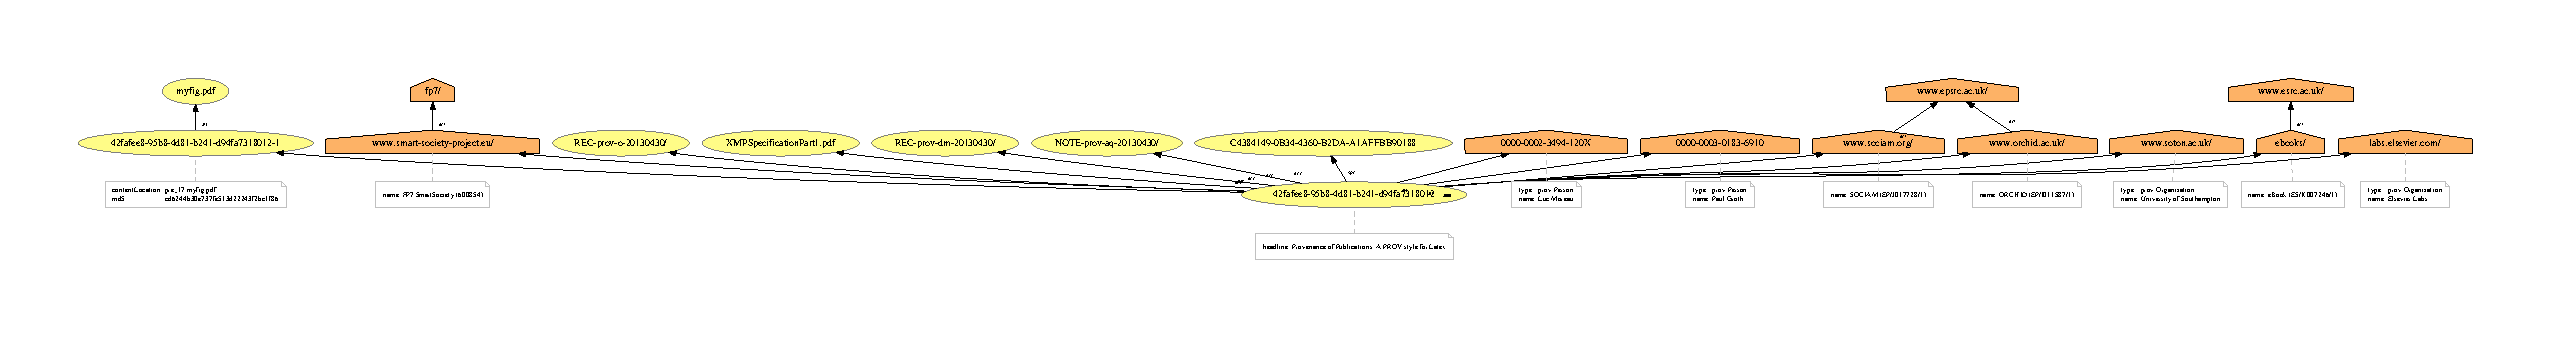
\includegraphics[angle=90,height=0.45\paperheight,origin=c]{myfig.pdf}
\caption{A Graphical Illustration of the Provenance of the Current Document.  The annotations indicate which \provsty macro underpinned the generation of which part of the graph. Vector graphics make this figure zoomable. The final version of the paper will also point to online version of the figure.}\label{prov:fig}  
\end{figure*}    

The overall provenance graph is rooted at this resource, appearing at
the bottom of the figure.  Annotations in the figure indicate which
\provsty macro was used to generate which portion of the graph.

We have refrained from designing our own ontology for expressing this
provenance. Instead, we relied on existing vocabularies, such as
\href{http://schema.org}{schema.org},
\href{Whehttp://xmlns.com/foaf/spec/}{foaf}, and a cryptography
ontology \href{http://www.w3.org/2000/10/swap/crypto/}{crypto}.

While most of the modelling in \PROV is straightforward, the
bibliography raises an interesting issue. Currently, a citation is
modeled by a \PROV derivation, to express that the current document
was derived from the cited document: derivation is to be understood as
building on, improving over, or addressing a problem differently than
previous work.  In the day-to-day practice of the scientific
community, it is possible for two documents to cite each other. This
would result in a cycle of derivation, which is regarded as invalid
provenance.

\section{Discussion}

With this paper, we have showed that it is possible to lower \PROV's
barrier of adoption, by adapting tools to generate provenance
automatically.  For those tools to be useful, they need to generate
provenance systematically, for every created artifact. Over time, as
similar tools get developed, their provenance should be linked up. For
instance, the \href{http://git2prov.org/}{git2prov} converter is
capable of exporting \PROV from GIT.  It should be possible for users
to seamleassly navigate the provenance generated by both tools.

While the \provsty style is still a proof of concept, we feel that it
is time to release it, and have others to use it.  Improving
usability, enhancing the quality of provenance, and strengthening of
\LaTeX\ integration are all desirable.  \provsty is available at
\provstyurl.

While it is great for metadata about the provenance to be embedded in
the PDF using XMP, it would have been nice to embed the provenance
itself. However, despite supporting RDF/XML, XMP imposes limitations
on the metadata content, and does not allow arbitrary \PROV graphs to
be embedded.




\acks

This work is funded in part by the EPSRC \provProject{SOCIAM (EP/J017728/1)}{http://www.sociam.org/}{http://www.epsrc.ac.uk/} and
\provProject{ORCHID (EP/I011587/1)}{http://www.orchid.ac.uk/}{http://www.epsrc.ac.uk/} projects, 
the \provProject{FP7 SmartSociety (600854)}{http://www.smart-society-project.eu/}{http://cordis.europa.eu/fp7/} project,
and the ESRC 
\provProject{eBook (ES/K007246/1)}{http://www.bristol.ac.uk/cmm/research/ebooks/}{http://www.esrc.ac.uk/} project.  




\provBibliography

% We recommend abbrvnat bibliography style.


\bibliographystyle{abbrvnat}
\bibliography{prov-sty-userguide}

\provEmbed

\end{document}

